\documentclass[12pt]{ctexart}
% set the left/right margin such that the main title can be written within one line
\usepackage[left=30mm]{geometry}
\usepackage{enumitem}
\AddEnumerateCounter{\chinese}{\chinese}{}
\usepackage{fancyhdr}
\usepackage{graphicx}
\usepackage{amssymb}
\usepackage{longtable}
\usepackage{multicol}
\usepackage{hyperref}
\usepackage{subcaption}
\fancypagestyle{runningpage}
{
  \fancyhead{}
    \fancyhead[L]{} 
    \fancyhead[C]{TPH-LINK 技术交流组}
    \fancyhead[R]{
\includegraphics[height=18pt]{tph-link.jpg}} 
  \fancyfoot{}
  \fancyfoot[C]{第 \thepage 页}
}
% not works?
\ctexset {
 appendixname = {附录}
}
\def\CurriculumScheduleWidth{1.6cm}
\begin{document}
% first page is cover
\title{
    \vspace{-0.5in}
    \textmd{\textbf{\huge{TPH-LINK技术交流组}}}\\
    \normalsize\vspace{0.1in}\Large{2018年秋季学期}\\
    \vspace{1in}
     \textbf{\huge{简}}\\
    \vspace{1in}
     \textbf{\huge{介}}\\
    \vspace{1in}
}
\author{赵丰}
\maketitle
\thispagestyle{empty}
\pagebreak
\pagestyle{runningpage}
\tableofcontents

\section{组织背景}
TPH-LINK ,全称深圳大学城三校(清华北大哈工大)交流协会,是由三校部分社团组织负责人发起的学生组织,成立于2018年9月2日。其中T是Tsinghua的首字母,P是Peking的首字母, H是Harbin的首字母。微信公众号“TPH\_LINK”。

TPH-LINK 技术交流组是TPH-LINK下的一个部门,致力于为IT专业的同学打造一个学习交流的平台。
TPH-LINK 技术交流组目前已经开展的活动有“微沙龙分享活动”和Tensorflow学习小组。计划开展的活动有
微信小程序线下培训或开发小组。

TPH-LINK 技术交流组与清华深研院科学技术协会与研会学术部均有密切的合作。


\section{微沙龙分享活动}
本学期10月13日至11月4日四周时间共开展5次微沙龙活动,请有经验的学长学姐主讲,内容涉及深度学习入门、对抗生成网络以及GitHub的使用等。

\begin{figure}[!ht]
\centering
  \begin{subfigure}[b]{0.4\textwidth}
  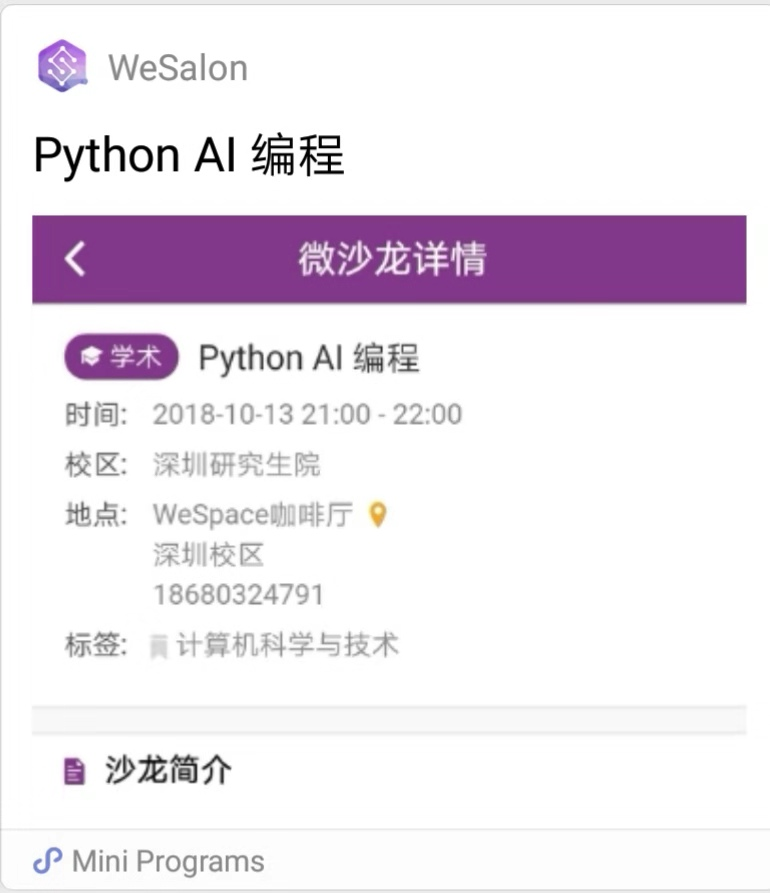
\includegraphics[width=\textwidth]{1/1.jpeg}  
    \end{subfigure}~
      \begin{subfigure}[b]{0.5\textwidth}
  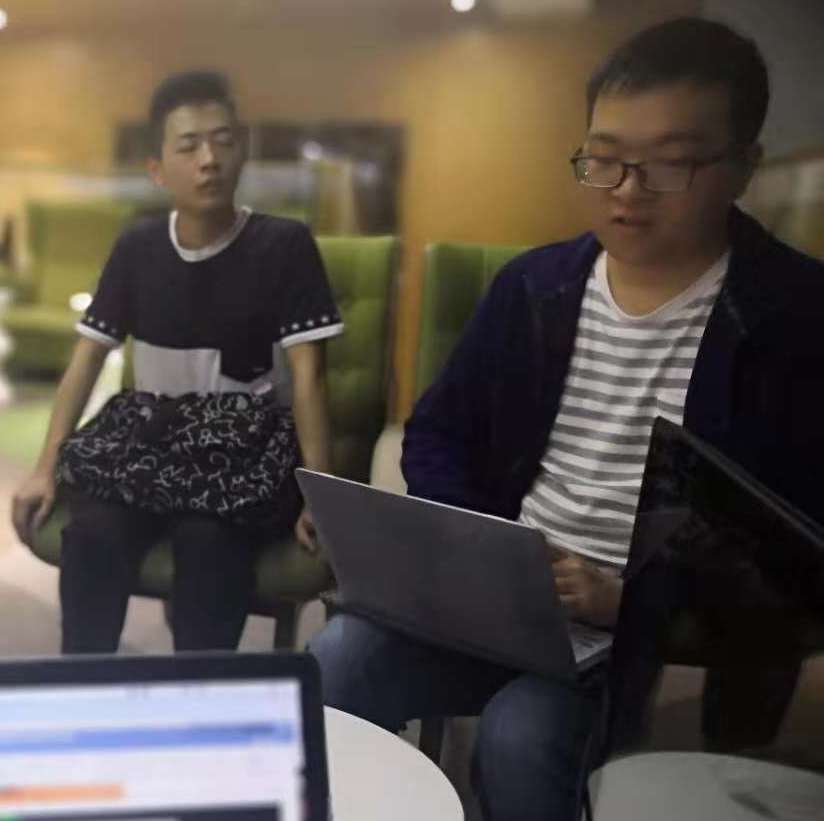
\includegraphics[width=\textwidth]{1/wesalon.jpeg}  
    \end{subfigure}
    \caption{第一次微沙龙分享}
\end{figure}
\begin{figure}[!ht]
\centering
  \begin{subfigure}[b]{0.4\textwidth}
  
\includegraphics[width=\textwidth]{2/2.jpeg}  
    \end{subfigure}~
      \begin{subfigure}[b]{0.5\textwidth}
  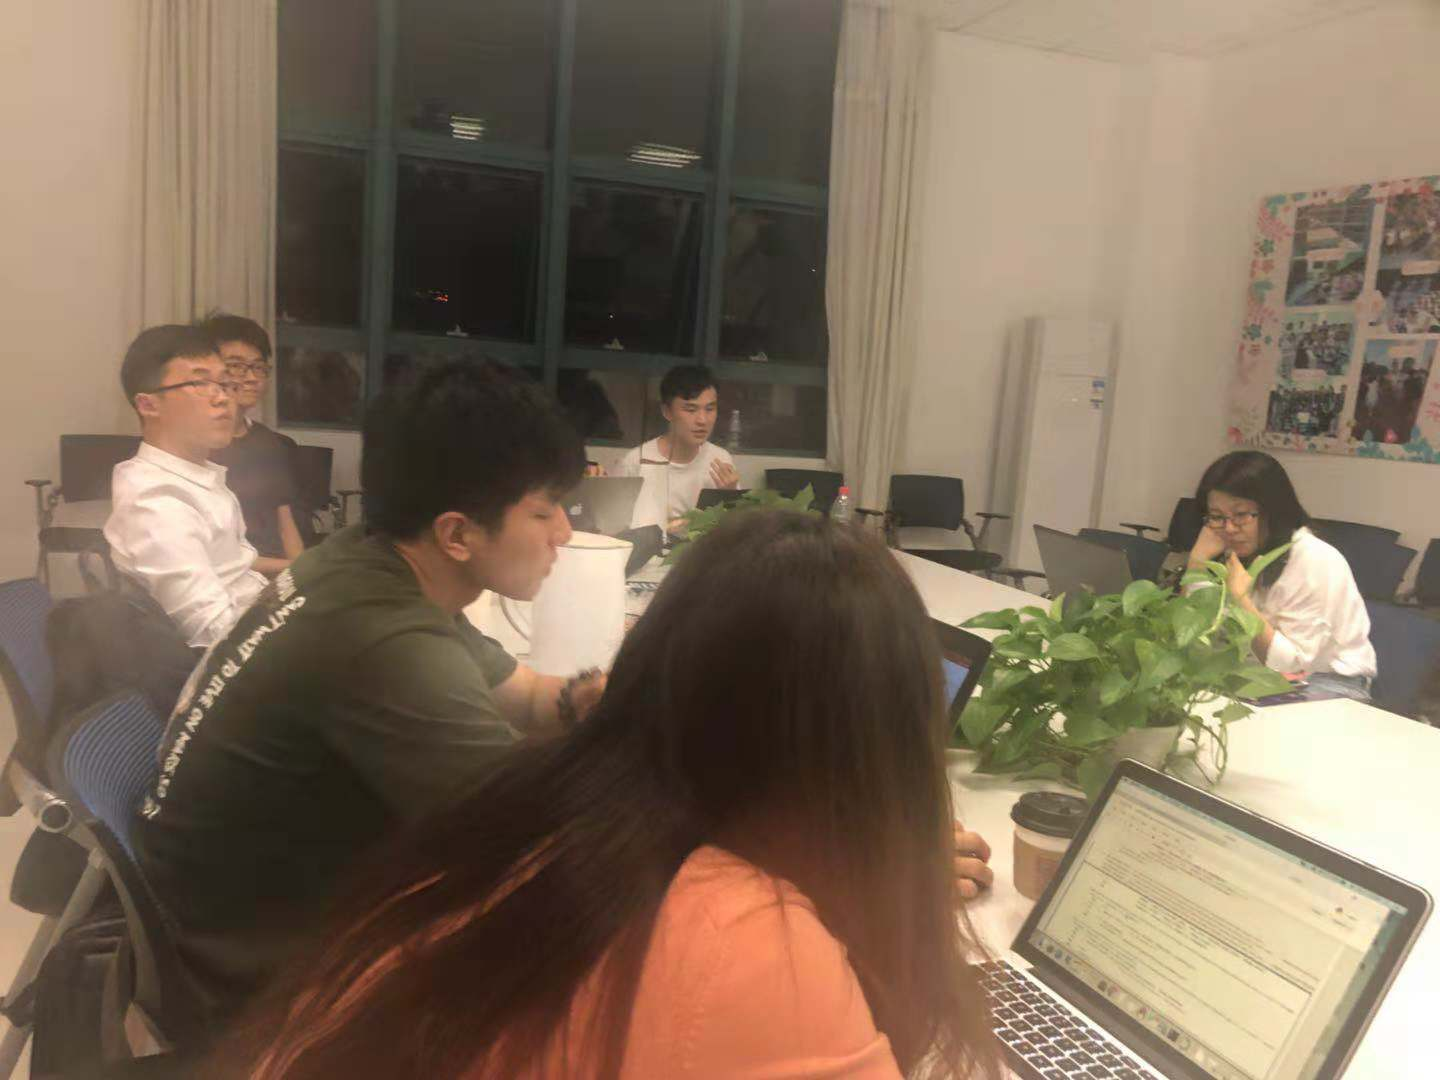
\includegraphics[width=\textwidth]{2/wesalon.jpeg}  
    \end{subfigure}
    \caption{第二次微沙龙分享}    
\end{figure}
\begin{figure}[!ht]
\centering
  \begin{subfigure}[b]{0.4\textwidth}
  
\includegraphics[width=\textwidth]{3/3.jpeg}  
    \end{subfigure}~
      \begin{subfigure}[b]{0.5\textwidth}
  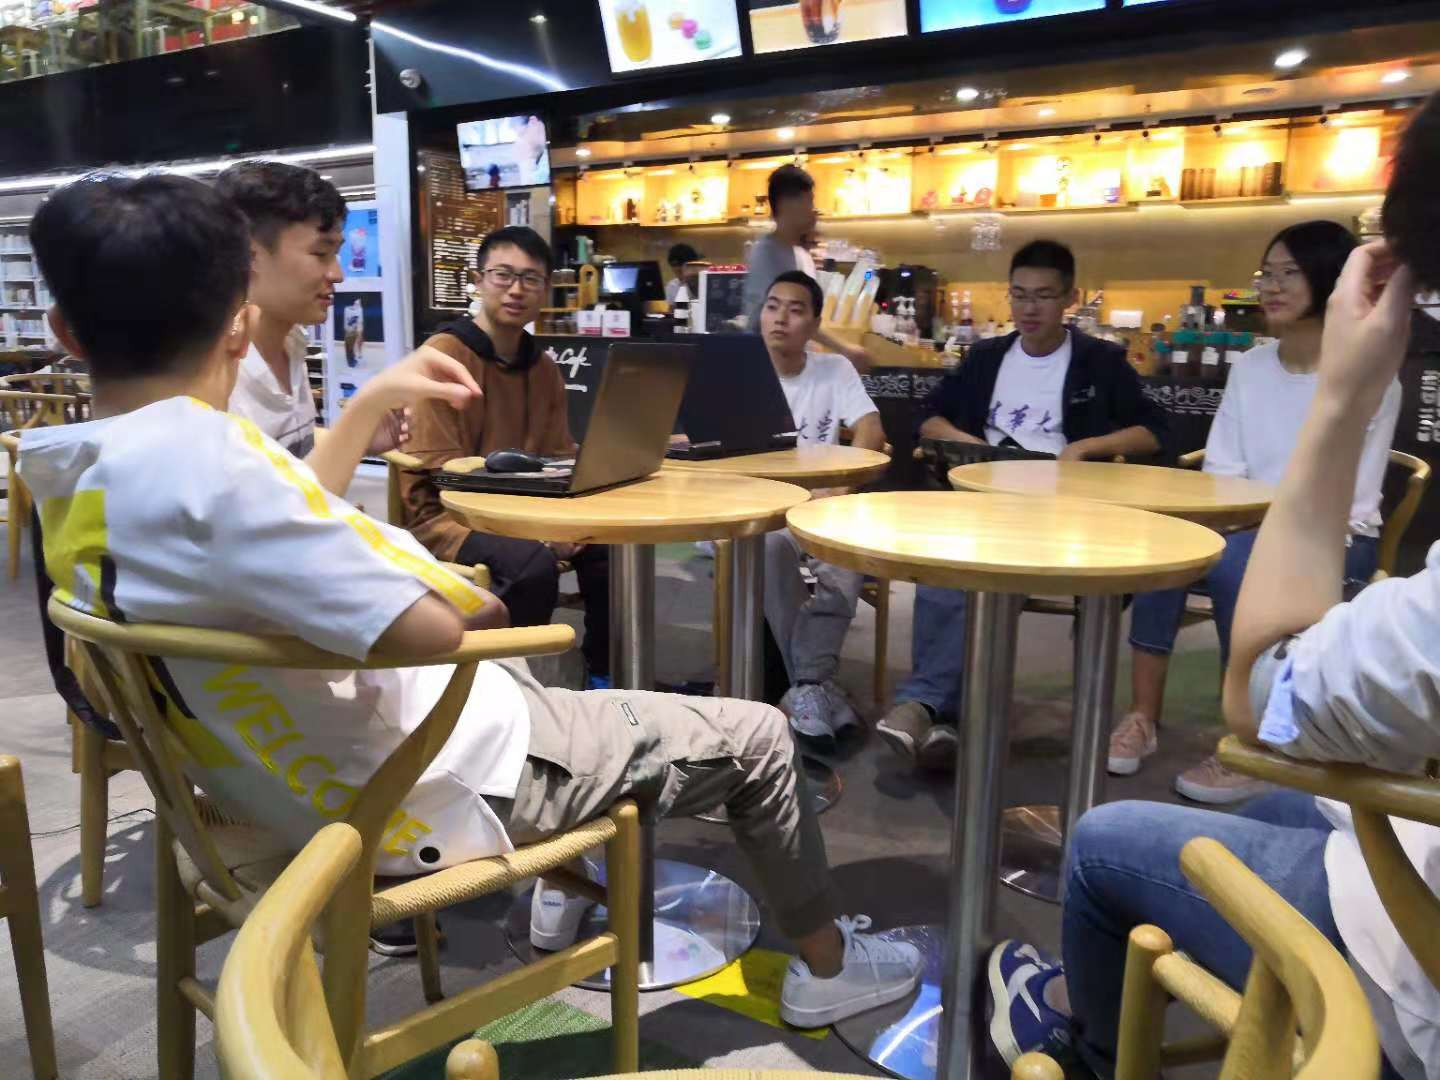
\includegraphics[width=\textwidth]{3/wesalon.jpeg}  
    \end{subfigure}
    \caption{第三次微沙龙分享}        
\end{figure}
\begin{figure}[!ht]
\centering
  \begin{subfigure}[b]{0.4\textwidth}
  
\includegraphics[width=\textwidth]{4/4.jpeg}  
    \end{subfigure}~
      \begin{subfigure}[b]{0.5\textwidth}
  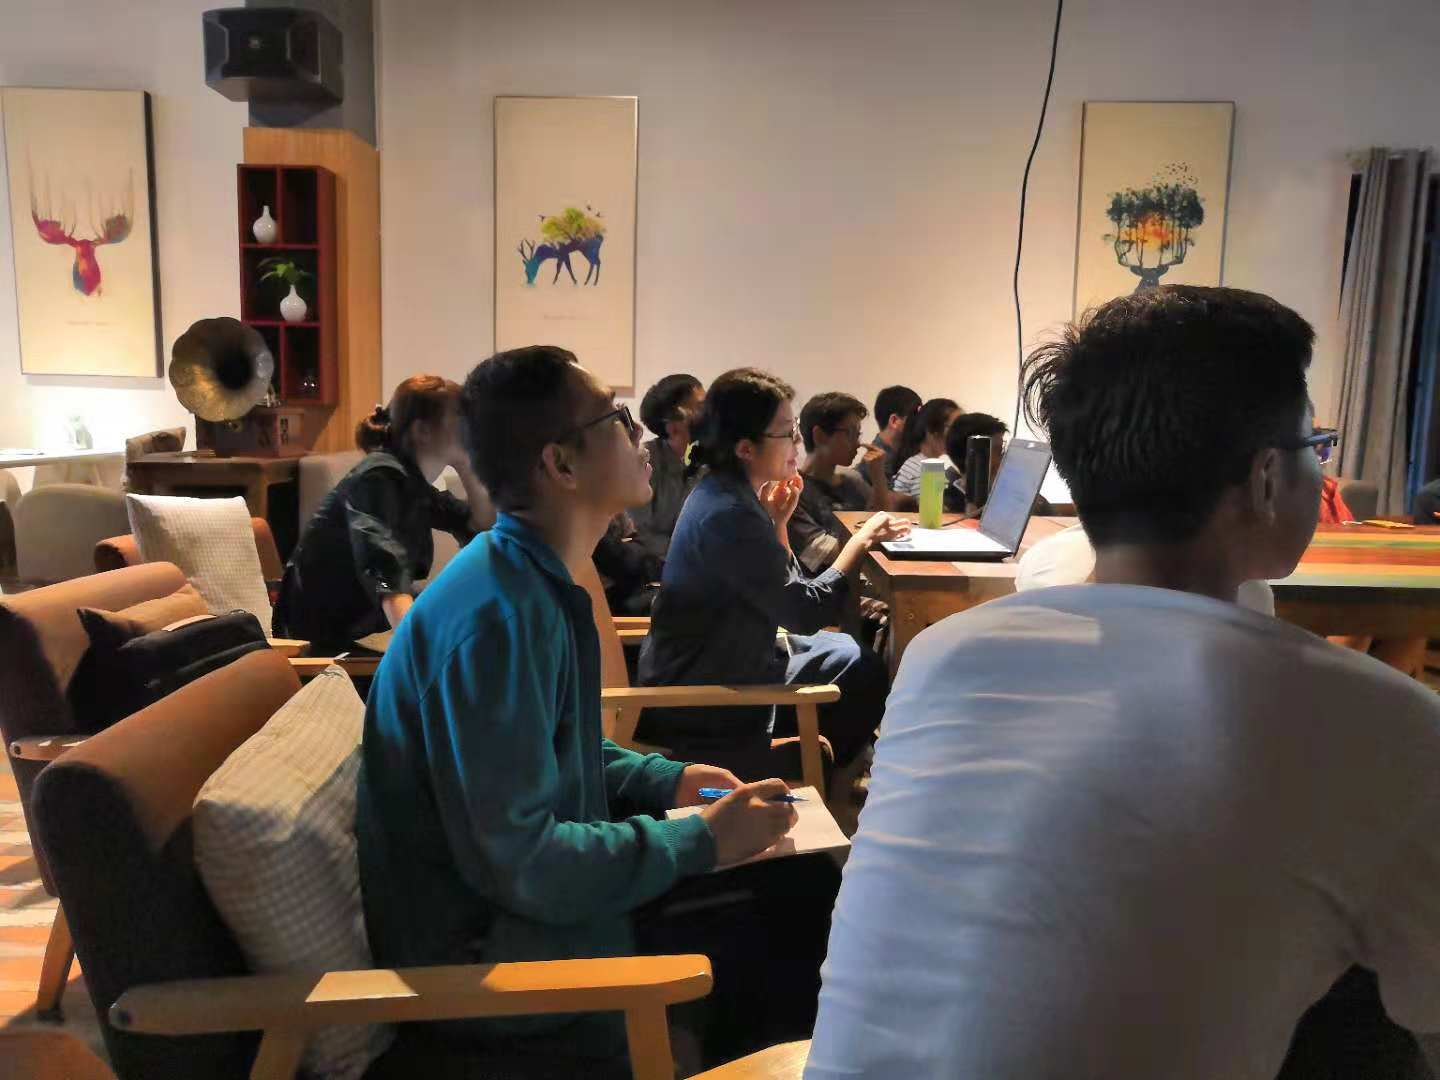
\includegraphics[width=\textwidth]{4/wesalon.jpg}  
    \end{subfigure}
    \caption{第四次微沙龙分享}        
\end{figure}
\begin{figure}[!ht]
\centering
  \begin{subfigure}[b]{0.4\textwidth}
  
\includegraphics[width=\textwidth]{5/poster.jpg}  
    \end{subfigure}~
      \begin{subfigure}[b]{0.5\textwidth}
  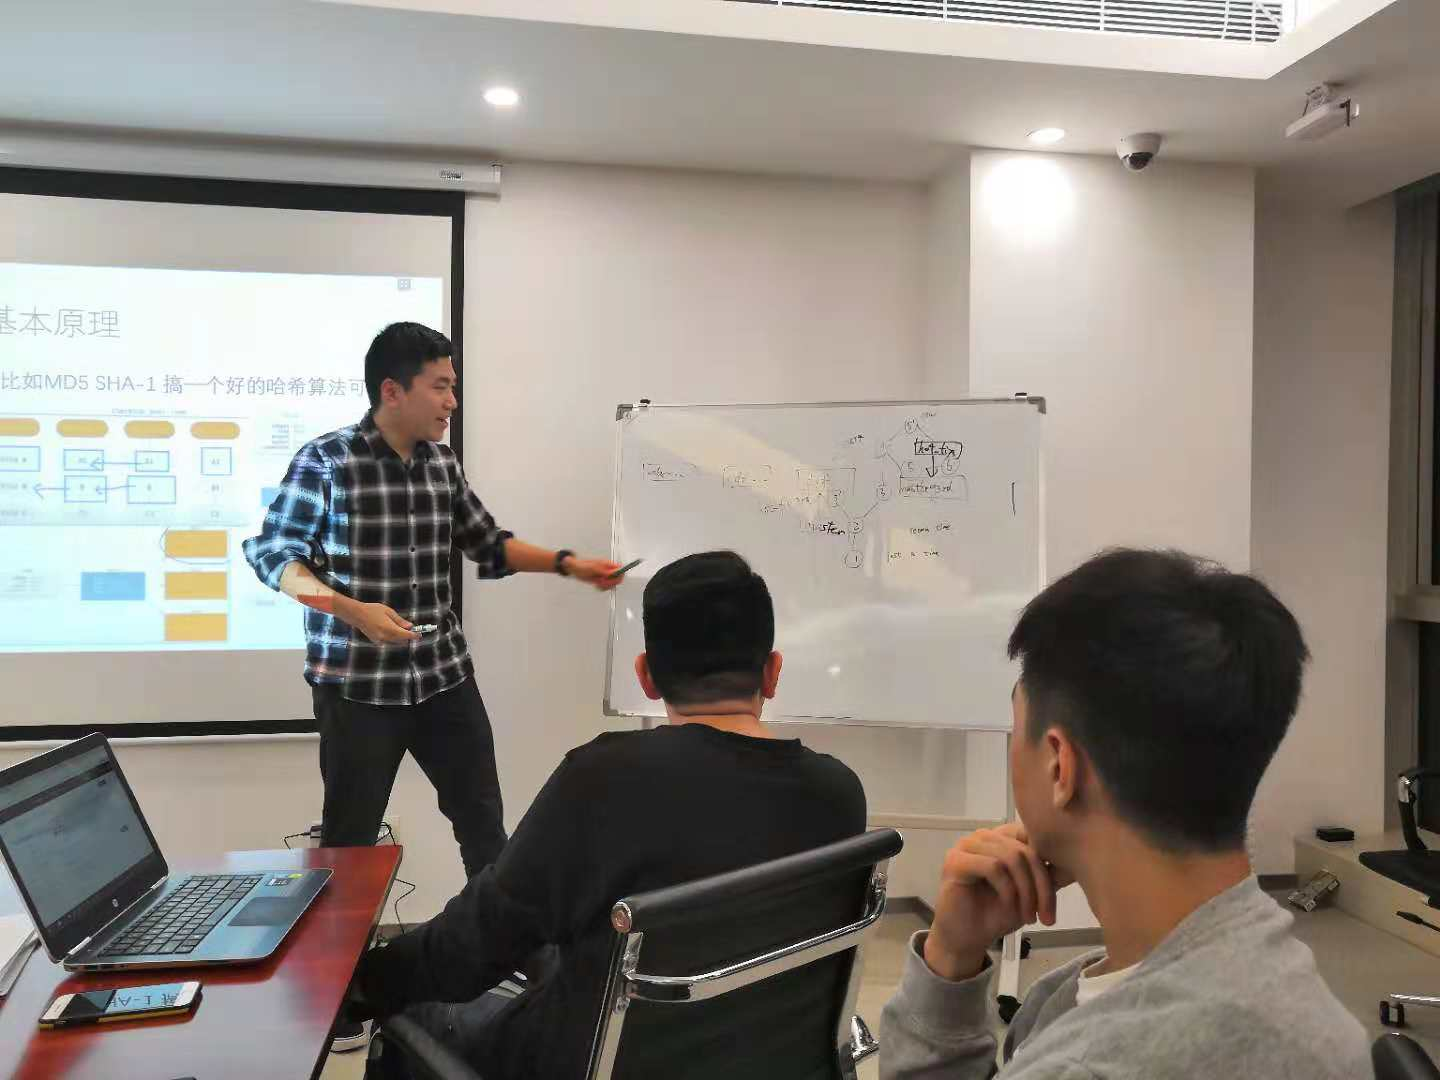
\includegraphics[width=\textwidth]{5/wesalon.jpeg}  
    \end{subfigure}
    \caption{第五次微沙龙分享}        
\end{figure}
\section{Tensorflow学习小组}
采用每两周一次线下聚会的形式,参与者轮流讲《TensorFlow实战Google深度学习框架》其中一章。目前已经进行了首次见面会(图\ref{tensorflow})。
\begin{figure}[!ht]
\centering
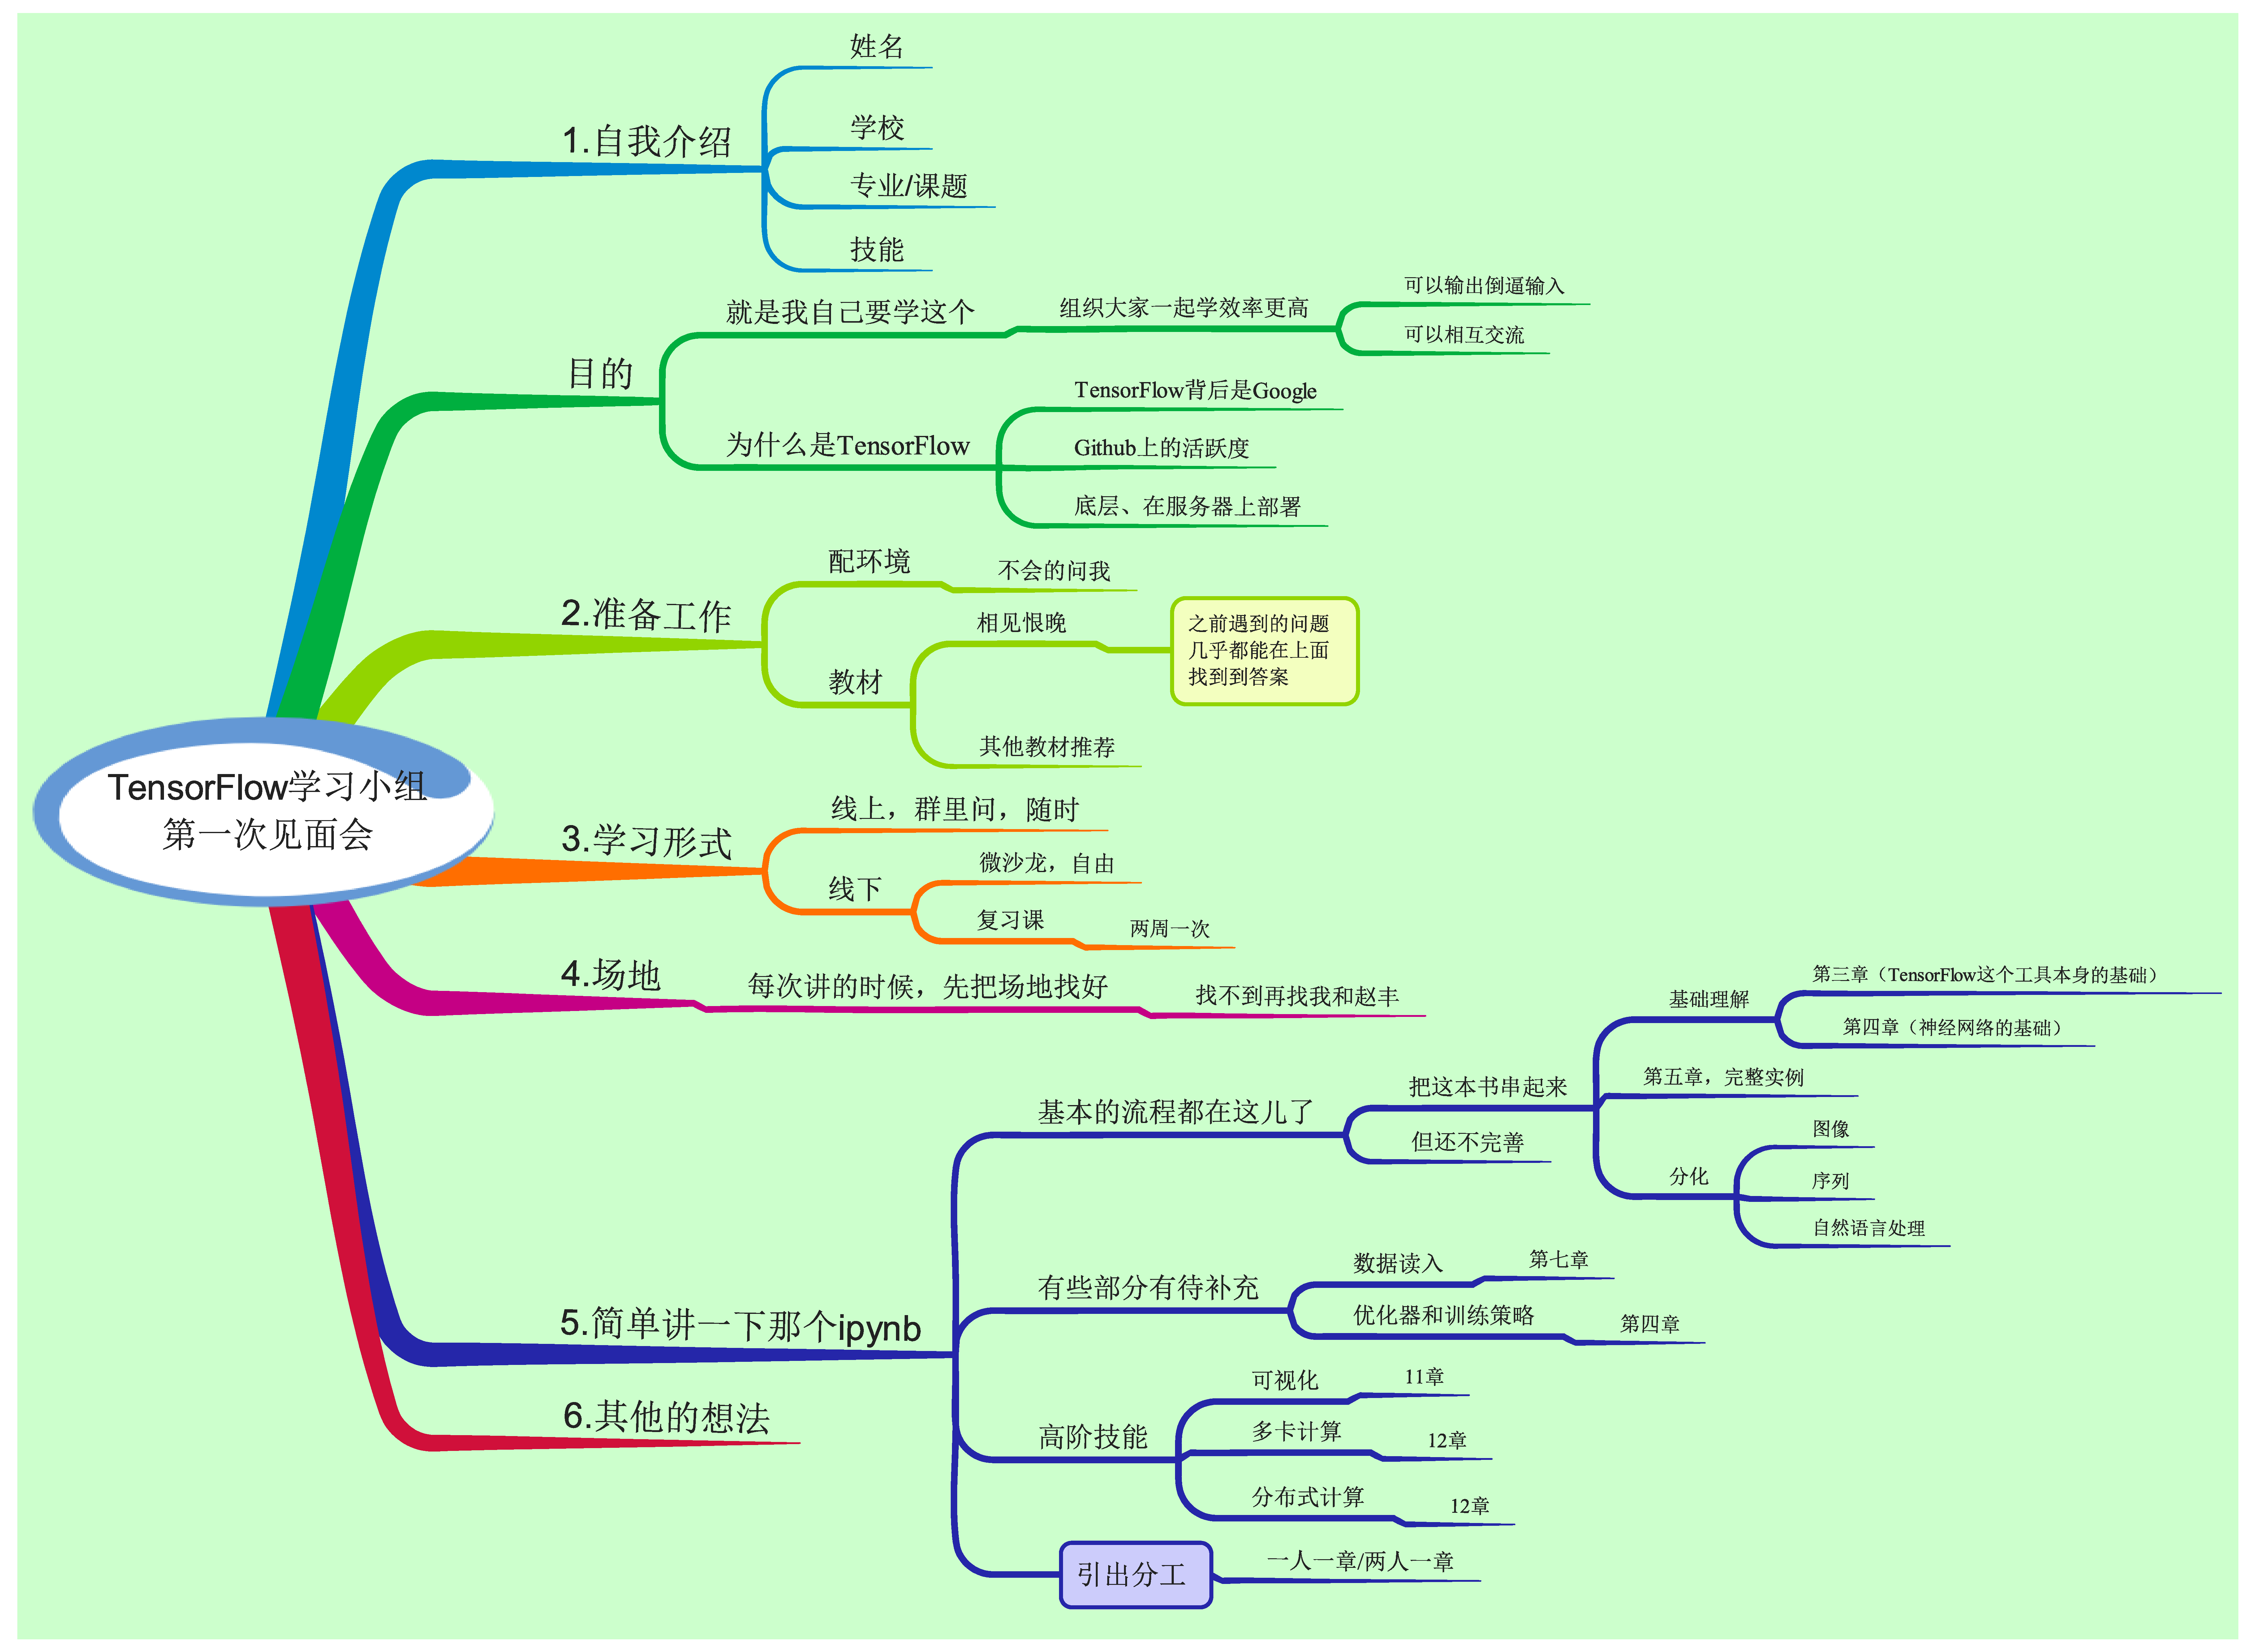
\includegraphics[width=12cm]{tensorflow_plan.pdf}
\caption{Tensorflow学习小组第一次见面会提要}        
\end{figure}
\begin{figure}[!ht]
\centering
  \begin{subfigure}[b]{0.4\textwidth}
  
\includegraphics[width=\textwidth]{qrcode.jpg}
  \subcaption{TPH-LINk公众号二维码}  
    \end{subfigure}~
      \begin{subfigure}[b]{0.5\textwidth}
  
\includegraphics[width=\textwidth]{tensorflow_first.jpg}  
  \subcaption{Tensorflow学习小组首次见面会} \label{tensorflow} 
    \end{subfigure}
\end{figure}
\section{微信小程序线下培训或开发小组}
在筹。
\end{document}

